\documentclass[12pt,a4paper]{article}
\usepackage{amsmath,amssymb,mathrsfs,tikz,times,pifont}
\usepackage{enumitem}
\newcommand\circitem[1]{%
\tikz[baseline=(char.base)]{
\node[circle,draw=gray, fill=red!55,
minimum size=1.2em,inner sep=0] (char) {#1};}}
\newcommand\boxitem[1]{%
\tikz[baseline=(char.base)]{
\node[fill=cyan,
minimum size=1.2em,inner sep=0] (char) {#1};}}
\setlist[enumerate,1]{label=\protect\circitem{\arabic*}}
\setlist[enumerate,2]{label=\protect\boxitem{\alph*}}
%%%::::::by chnini ameur :::::::%%%
\everymath{\displaystyle}
\usepackage[left=1cm,right=1cm,top=1cm,bottom=1.7cm]{geometry}
\usepackage[colorlinks=true, linkcolor=blue, urlcolor=blue, citecolor=blue]{hyperref}
\usepackage{array,multirow}
\usepackage[most]{tcolorbox}
\usepackage{varwidth}
\usepackage{float} %pour utiliser l'option [H] qui force l'image à apparaître exactement à l'endroit où elle est placée dans le code.
\tcbuselibrary{skins,hooks}
\usetikzlibrary{patterns}
%%%::::::by chnini ameur :::::::%%%
\newtcolorbox{exa}[2][]{enhanced,breakable,before skip=2mm,after skip=5mm,
colback=yellow!20!white,colframe=black!20!blue,boxrule=0.5mm,
attach boxed title to top left ={xshift=0.6cm,yshift*=1mm-\tcboxedtitleheight},
fonttitle=\bfseries,
title={#2},#1,
% varwidth boxed title*=-3cm,
boxed title style={frame code={
\path[fill=tcbcolback!30!black]
([yshift=-1mm,xshift=-1mm]frame.north west)
arc[start angle=0,end angle=180,radius=1mm]
([yshift=-1mm,xshift=1mm]frame.north east)
arc[start angle=180,end angle=0,radius=1mm];
\path[left color=tcbcolback!60!black,right color = tcbcolback!60!black,
middle color = tcbcolback!80!black]
([xshift=-2mm]frame.north west) -- ([xshift=2mm]frame.north east)
[rounded corners=1mm]-- ([xshift=1mm,yshift=-1mm]frame.north east)
-- (frame.south east) -- (frame.south west)
-- ([xshift=-1mm,yshift=-1mm]frame.north west)
[sharp corners]-- cycle;
},interior engine=empty,
},interior style={top color=yellow!5}}
%%%%%%%%%%%%%%%%%%%%%%%

\usepackage{fancyhdr}
\usepackage{eso-pic}         % Pour ajouter des éléments en arrière-plan
% Commande pour ajouter du texte en arrière-plan
\usepackage{tkz-tab}
\AddToShipoutPicture{
    \AtTextCenter{%
        \makebox[0pt]{\rotatebox{80}{\textcolor[gray]{0.5}{\fontsize{5cm}{5cm}\selectfont PGB}}}
    }
}
\usepackage{lastpage}
\fancyhf{}
\pagestyle{fancy}
\renewcommand{\footrulewidth}{1pt}
\renewcommand{\headrulewidth}{0pt}
\renewcommand{\footruleskip}{10pt}
\fancyfoot[R]{
\color{blue}\ding{45}\ \textbf{2025}
}
\fancyfoot[L]{
\color{blue}\ding{45}\ \textbf{Prof:M. BA}
}
\cfoot{\bf
\thepage /
\pageref{LastPage}}
% Définition de l'encadré adaptatif avec fond jaune
\newtcolorbox{resultbox}{
    colback=red!30, % Fond rouge clair
    colframe=black, % Bordure noire fine
    sharp corners, % Coins nets
    boxrule=0.5pt, % Contour léger
    boxsep=2pt, % Espacement interne
    left=5pt, right=5pt, top=2pt, bottom=2pt, % Marges internes
}
\begin{document}
\renewcommand{\arraystretch}{1.5}
\renewcommand{\arrayrulewidth}{1.2pt}
\begin{tikzpicture}[overlay,remember picture]
\node[draw=blue,line width=1.2pt,fill=purple,text=blue,inner sep=3mm,rounded corners,pattern=dots]at ([yshift=-2.5cm]current page.north) {\begingroup\setlength{\fboxsep}{0pt}\colorbox{white}{\begin{tabular}{|*1{>{\centering \arraybackslash}p{0.28\textwidth}} |*2{>{\centering \arraybackslash}p{0.2\textwidth}|} *1{>{\centering \arraybackslash}p{0.19\textwidth}|} }
\hline
\multicolumn{3}{|c|}{$\diamond$$\diamond$$\diamond$\ \textbf{Lycée de Dindéfélo}\ $\diamond$$\diamond$$\diamond$ }& \textbf{A.S. : 2024/2025} \\ \hline
\textbf{Matière: Mathématiques}& \textbf{Niveau : 2}\textbf{ndL} &\textbf{Date: 16/06/2025} & \textbf{Durée : 3 heures} \\ \hline
\multicolumn{4}{|c|}{\parbox[c]{10cm}{\begin{center}
\textbf{{\Large\sffamily Correction de la composition Du 2$ ^\text{\bf nd} $ Semestre}}
\end{center}}} \\ \hline
\end{tabular}}\endgroup};
\end{tikzpicture}
\vspace{3cm}

\section*{\underline{Correction Exercice 1 :} 4 pts }

\begin{enumerate}
    \item Résolution algébrique du système : \hfill \textbf{2 pts}
    
    \[
    \left\{
    \begin{aligned}
        2x + y &= 3 \quad \text{(1)} \\
        3x + 2y &= 6 \quad \text{(2)}
    \end{aligned}
    \right.
    \]

    \textbf{Méthode : substitution (ou addition)}

    De (1) : \( y = 3 - 2x \)

    On remplace dans (2) :

    \[
    \begin{aligned}
    3x + 2(3 - 2x) &= 6 \\
    3x + 6 - 4x &= 6 \\
    -x + 6 &= 6 \\
    -x &= 0 \quad \Rightarrow \quad x = 0
    \end{aligned}
    \]

    On remplace \( x = 0 \) dans (1) : \( 2 \cdot 0 + y = 3 \Rightarrow y = 3 \)

     \begin{resultbox}
    \[
    \mathbf{S =\{(0;3)\}}
    \]
		\end{resultbox}

    \item Résolution graphique du système : \hfill \textbf{2 pts}

    \textbf{Cramer}

    \section*{Résolution par la méthode de Cramer}

On considère le système :
\[
\left\{
\begin{aligned}
2x + y &= 3 \\
3x + 2y &= 6
\end{aligned}
\right.
\]

On note :
\[
\Delta = 
\begin{vmatrix}
2 & 1 \\
3 & 2
\end{vmatrix}
\qquad
\Delta_x = 
\begin{vmatrix}
3 & 1 \\
6 & 2
\end{vmatrix}
\qquad
\Delta_y = 
\begin{vmatrix}
1 & 3 \\
2 & 6
\end{vmatrix}
\]

\[
\Delta = 
\begin{vmatrix}
2 & 1 \\
3 & 2
\end{vmatrix}
=4-3=1
\]

\[
\Delta_x = 
\begin{vmatrix}
3 & 1 \\
6 & 2
\end{vmatrix}
=6-6=0
\]

\[
\Delta_y = 
\begin{vmatrix}
2 & 3 \\
3 & 6
\end{vmatrix}
=12-9=3
\]

\[x=\frac{\Delta_x}{\Delta} = \frac{0}{1} ; y=\frac{\Delta_y}{\Delta} = \frac{3}{1}\]

    \begin{resultbox}
    \[
    \mathbf{S =\{(0;3)\}}
    \]
		\end{resultbox}
\begin{center}
\begin{figure}[H]% Forcer l'image à cet endroit
\centering
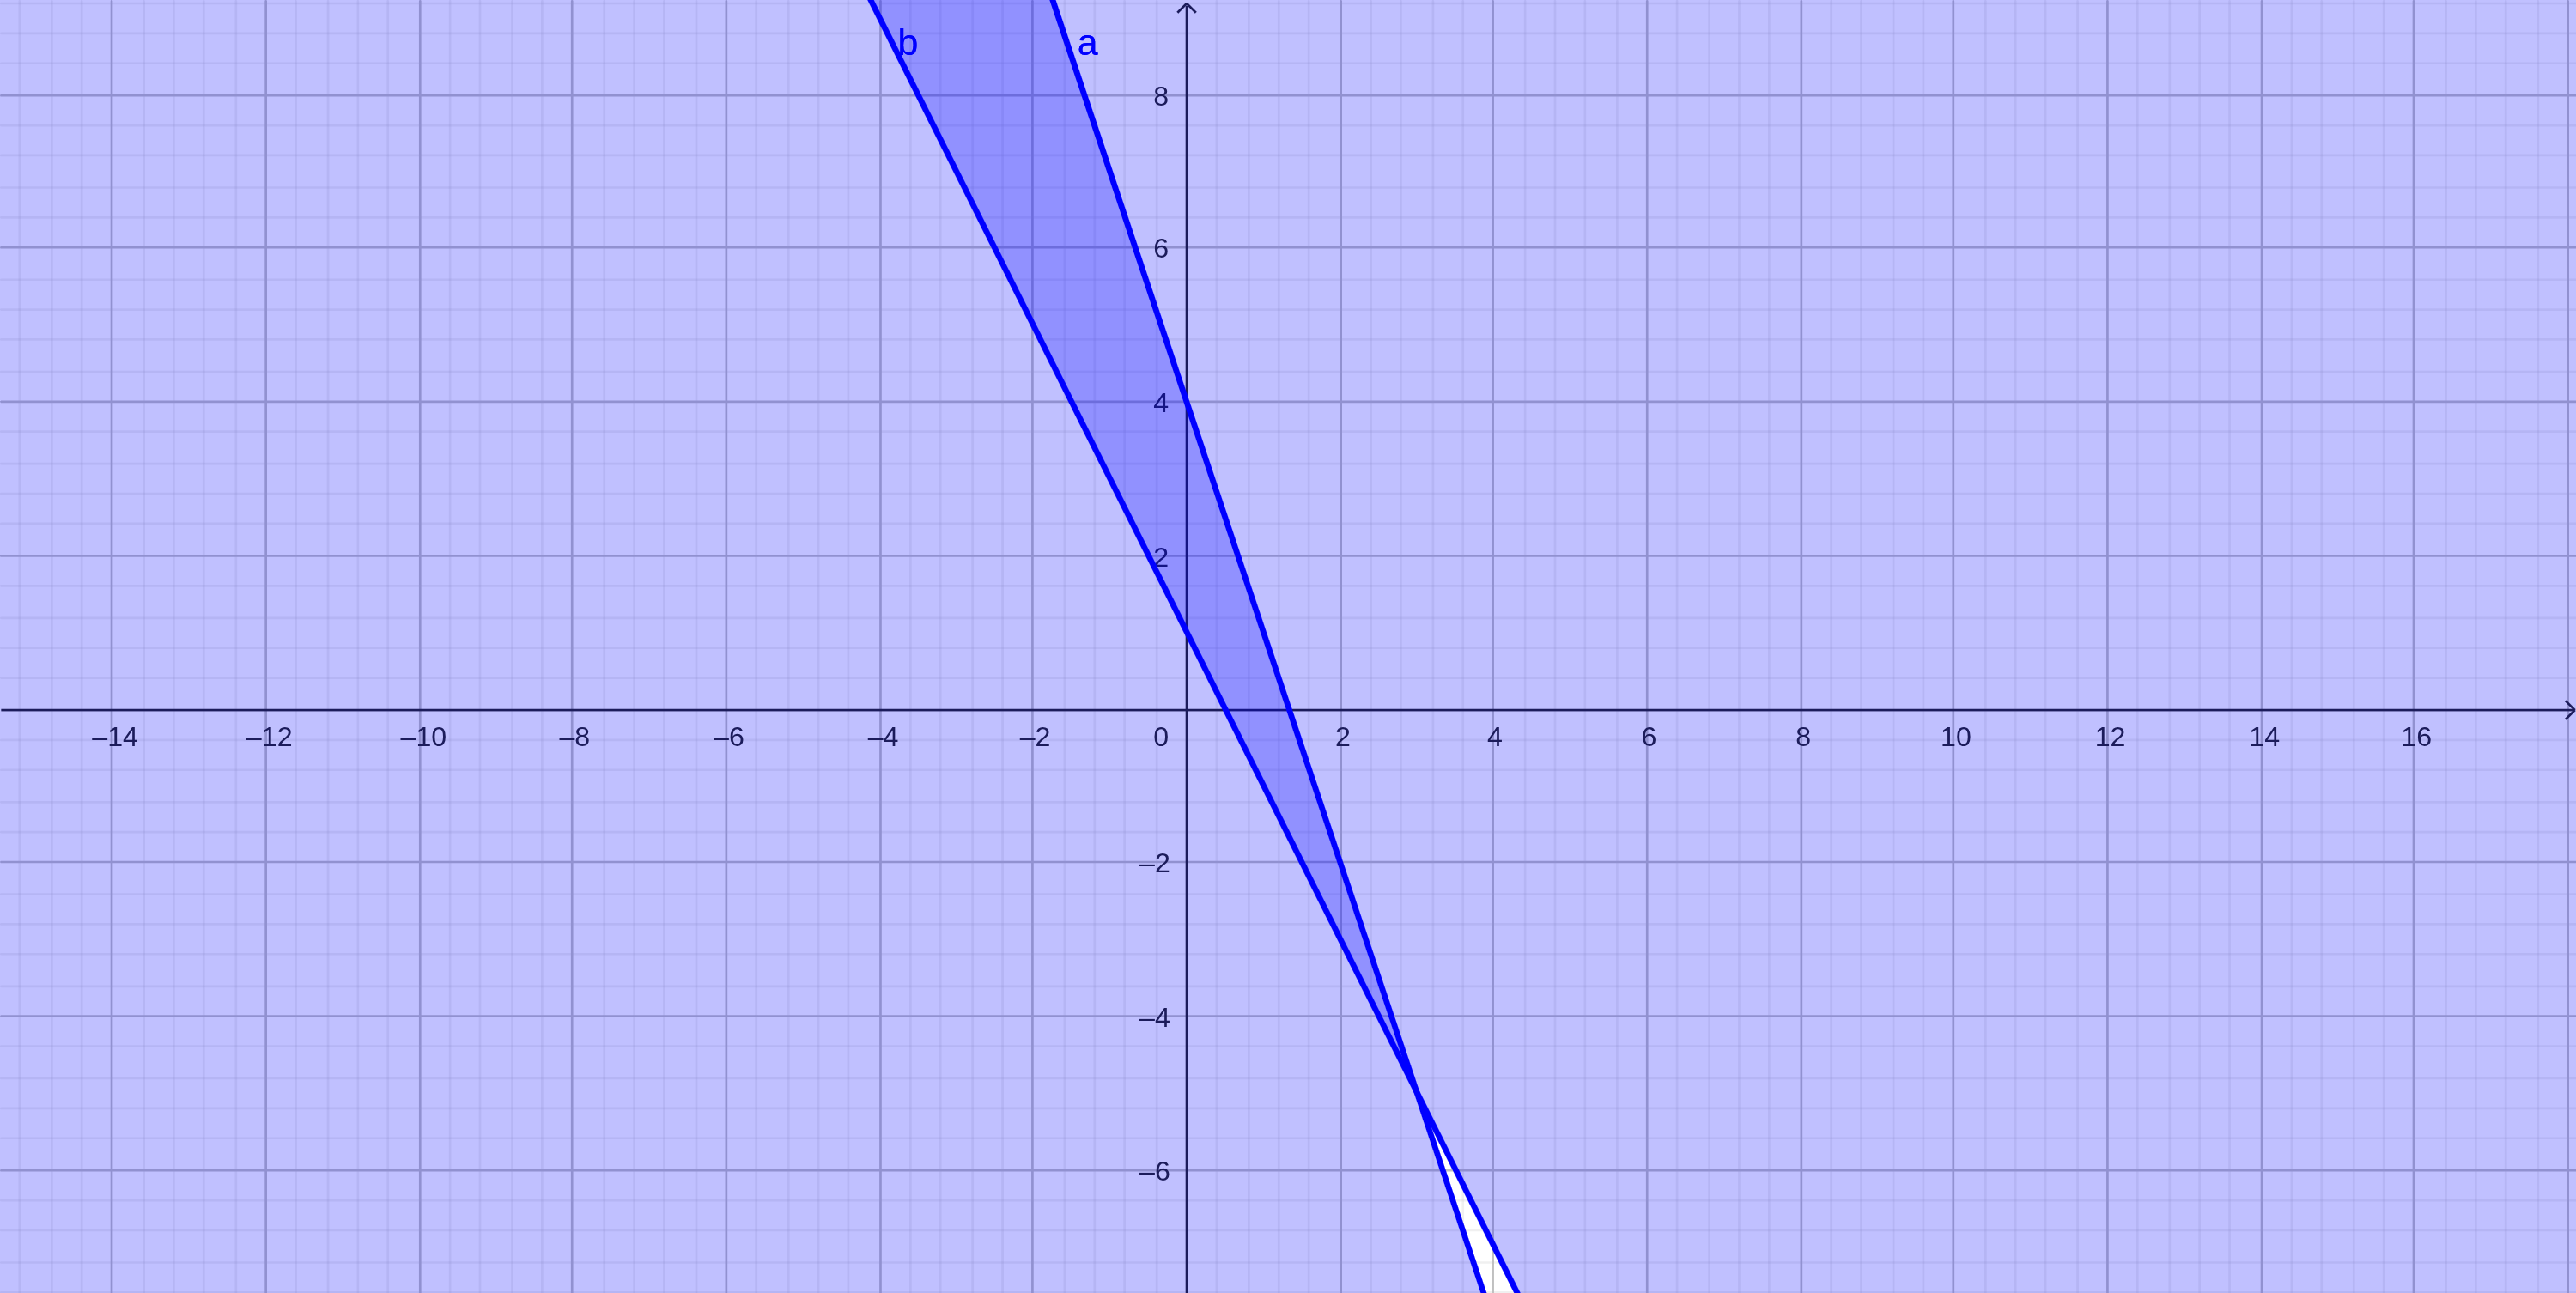
\includegraphics[width=0.8\textwidth]{Compo2ndL.png}
\caption{Représentation graphique du système}
\label{fig:monimage}
\end{figure}
\href{https://www.geogebra.org/classic/ebh2sxnk}{Clique ici pour voir la courbe sur géogébra}\\
\end{center}
\end{enumerate}

\section*{\underline{Correction Exercice 2 :} 8 pts}

\begin{enumerate}
    \item \textbf{Discriminant, forme canonique et factorisée} \hfill \textbf{3 pts}

    On considère le trinôme : \( f(x) = -2x^2 + 7x - 5 \)

    \textbf{Calcul du discriminant :}

    \[
    a = -2,\quad b = 7,\quad c = -5
    \]
    \[
    \Delta = b^2 - 4ac = 7^2 - 4 \times (-2) \times (-5) = 49 - 40 = 9
    \]

    \textbf{Forme canonique :}
    
    $
\begin{aligned}
    f(x)&= a \left[ \left(x + \frac{b}{2a}\right)^2 - \frac{b^{2}-4ac}{4a^{2}}\right]\\
    		&= a \left[ \left(x + \frac{b}{2a}\right)^2 - \frac{\Delta}{4a^{2}}\right]\\
        &= -2\left[ \left( x - \frac{7}{2(-2)} \right)^2 - \frac{9}{4(-2)^{2}} \right]\\
        &=-2\left[ \left( x - \frac{7}{-4} \right)^2 - \frac{9}{16} \right]\\
        &=-2\left[ \left( x + \frac{7}{4} \right)^2 - \frac{9}{16} \right]
\end{aligned}
$

    \begin{resultbox}
    \[
    \mathbf{f(x)=-2\left[ \left( x + \frac{7}{4} \right)^2 - \frac{9}{16} \right]}
    \]
		\end{resultbox}

    \textbf{Forme factorisée :}

    \[
    x_1 = \frac{-b - \sqrt{\Delta}}{2a} = \frac{-7 - 3}{-4} = \frac{-10}{-4} = \frac{5}{2}, \quad
    x_2 = \frac{-7 + 3}{-4} = \frac{-4}{-4} = 1
    \]
    
    \begin{resultbox}
    \[
    \mathbf{f(x) = -2(x - 1)\left(x - \frac{5}{2}\right)}
    \]
		\end{resultbox}

    \item \textbf{Résolution de l’équation} \( x^2 - 3x - 10 = 0 \) \hfill \textbf{1 pt}

    \[
    \Delta = (-3)^2 - 4 \cdot 1 \cdot (-10) = 9 + 40 = 49
    \Rightarrow \sqrt{\Delta} = 7
    \]

    \[
    x_1 = \frac{3 - 7}{2} = -2, \quad x_2 = \frac{3 + 7}{2} = 5
    \]
		
    \begin{resultbox}
    \[
    \mathbf{S=\{-2 ; 5\}}
    \]
		\end{resultbox}

    \item \textbf{Résolution de l’inéquation} \( x^2 - 3x - 10 \leq 0 \) \hfill \textbf{2 pts}

    On a déjà les racines : \( x = -2 \) et \( x = 5 \)

		
		\begin{center}
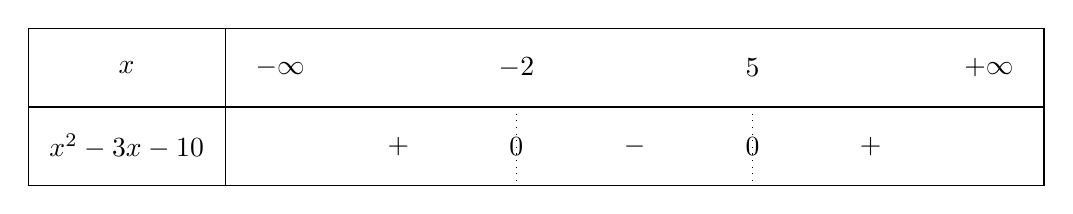
\begin{tikzpicture}
   \tkzTabInit[lgt = 2.5, espcl = 3, deltacl = 0.7]{$x$ / 1 , $x^2 - 3x - 10$ / 1 }{$-\infty$, $-2$,$5$, $+\infty$}
   \tkzTabLine{, + , z ,-,z, + }
\end{tikzpicture}

\end{center}
    \begin{resultbox}
    \[
    \mathbf{S=[-2\,;\,5]}
    \]
\end{resultbox}

    \item \textbf{Résolution du système} \hfill \textbf{2 pts}
    \[
    \left\{
    \begin{aligned}
        x + y &= -5 \quad \text{(1)}\\
        x \times y &= 6 \quad \text{(2)}
    \end{aligned}
    \right.
    \]

\begin{center}
\textbf{Première Mèthode}
\end{center}

\section*{Résolution du système}

Résolvons le système suivant :
\[
\left\{
\begin{aligned}
x + y &= -5 \quad \text{(1)}\\
x \cdot y &= 6 \quad \text{(2)}
\end{aligned}
\right.
\]

\textbf{Étape 1 :} Exprimer une variable à partir de l’équation (1) :  
\[
y = -5 - x
\]

\textbf{Étape 2 :} Remplacer dans (2) :
\[
x(-5 - x) = 6 \quad \Rightarrow \quad -5x - x^2 = 6 \quad \Rightarrow \quad x^2 + 5x + 6 = 0
\]

\textbf{Étape 3 :} Résolution du trinôme :
\[
\Delta = 5^2 - 4 \cdot 1 \cdot 6 = 25 - 24 = 1
\]
\[
x_1 = \frac{-5 - 1}{2} = -3 \quad ; \quad x_2 = \frac{-5 + 1}{2} = -2
\]

\textbf{Étape 4 :} Calcul des valeurs de \( y \) :

\begin{itemize}
    \item Si \( x = -3 \), alors \( y = -5 - (-3) = -2 \)
    \item Si \( x = -2 \), alors \( y = -5 - (-2) = -3 \)
\end{itemize}

\textbf{Solution finale :}
\[
\boxed{
(x, y) \in \{ (-3, -2),\ (-2, -3) \}
}
\]
\begin{center}
\textbf{Deuxième Mèthode}
\end{center}  

    \[
    \left\{
    \begin{aligned}
        x + y &= -5 \quad \text{(1)}\\
        x \times y &= 6 \quad \text{(2)}
    \end{aligned}
    \right.\implies
       \left\{
    \begin{aligned}
        S &= -5 \quad \text{(1)}\\
        P &= 6 \quad \text{(2)}
    \end{aligned}
    \right.
    \]    

\[
\text{Ce système est équivalente à : } X^2-SX+P = 0 \text{ donc } X^2+5X+6 = 0
\]    
    
    \begin{resultbox}
    \[
    \mathbf{S =\{(-3, -2),\ (-2, -3)\}}
    \]
		\end{resultbox}
\end{enumerate}

\section*{\underline{ Correction Exercice 3 :} 8 pts}

\subsection*{\underline{PARTIE A :} 5 pts}

On considère les fonctions suivantes :
\[
f(x) = -\frac{1}{2}x + 3 \quad ; \quad g(x) = 5x + 10 \quad ; \quad h(x) = 3
\]

\begin{enumerate}
    \item \textbf{Sens de variation} \hfill \textbf{1,5 pt}
    
    \begin{itemize}
        \item \( f(x) = -\frac{1}{2}x + 3 \) est une fonction affine de coefficient directeur ,$\textcolor{red}{-\frac{1}{2}<0}$, négatif  donc elle est \textbf{décroissante} sur \( \mathbb{R} \).
        \item \( g(x) = 5x + 10 \) est une fonction affine de coefficient directeur ,$\textcolor{red}{5>0}$, positif, donc elle est \textbf{croissante} sur \( \mathbb{R} \).
        \item \( h(x) = 3 \) est une fonction constante ,$\textcolor{red}{a=0}$, donc elle est \textbf{ni croissante ni décroissante}.
    \end{itemize}

    \item Soit \( k(x) = 3x + 2 \)
    \begin{enumerate}
        \item \textbf{Calcul de l’image de \(-1\) et de \(0\)} \hfill \textbf{1 pt}
        
        \[
        k(-1) = 3 \times (-1) + 2 = -3 + 2 = -1
        \]
        \[
        k(0) = 3 \times 0 + 2 = 0 + 2 = 2
        \]
        
     \begin{resultbox}
    \[
    \mathbf{k(-1) = -1 \quad ; \quad k(0) = 2}
    \]
		\end{resultbox}

        \item \textbf{Détermination des antécédents de \( 7 \) et \( \dfrac{1}{2} \)} \hfill \textbf{1 pt}

        Résolvons \( 3x + 2 = 7 \) :
        \[
        3x = 7 - 2 = 5 \quad \Rightarrow \quad x = \frac{5}{3}
        \]

        Résolvons \( 3x + 2 = \dfrac{1}{2} \) :
        \[
        3x = \frac{1}{2} - 2 = \frac{1}{2} - \frac{4}{2} = \frac{-3}{2} \quad \Rightarrow \quad x = -\frac{1}{2}
        \]

		\begin{resultbox}
    \[
    \mathbf{k^{-1}(7) = \frac{5}{3} \quad ; \quad k^{-1}\left(\frac{1}{2}\right) = -\frac{1}{2}}
    \]
		\end{resultbox}

        \item \textbf{Représentation graphique de \( k(x) = -3x + 2 \)} \hfill \textbf{1,5 pt}

        Deux points suffisent pour tracer la droite :
        \begin{itemize}
            \item Pour \( x = 0 \), \( k(0) = 2 \)  point \( (0\,;\,2) \)
            \item Pour \( x = 1 \), \( k(1) = -3 + 2 = -1 \)  point \( (1\,;\,-1) \)
        \end{itemize}

\begin{center}
\begin{figure}[H]% Forcer l'image à cet endroit
\centering
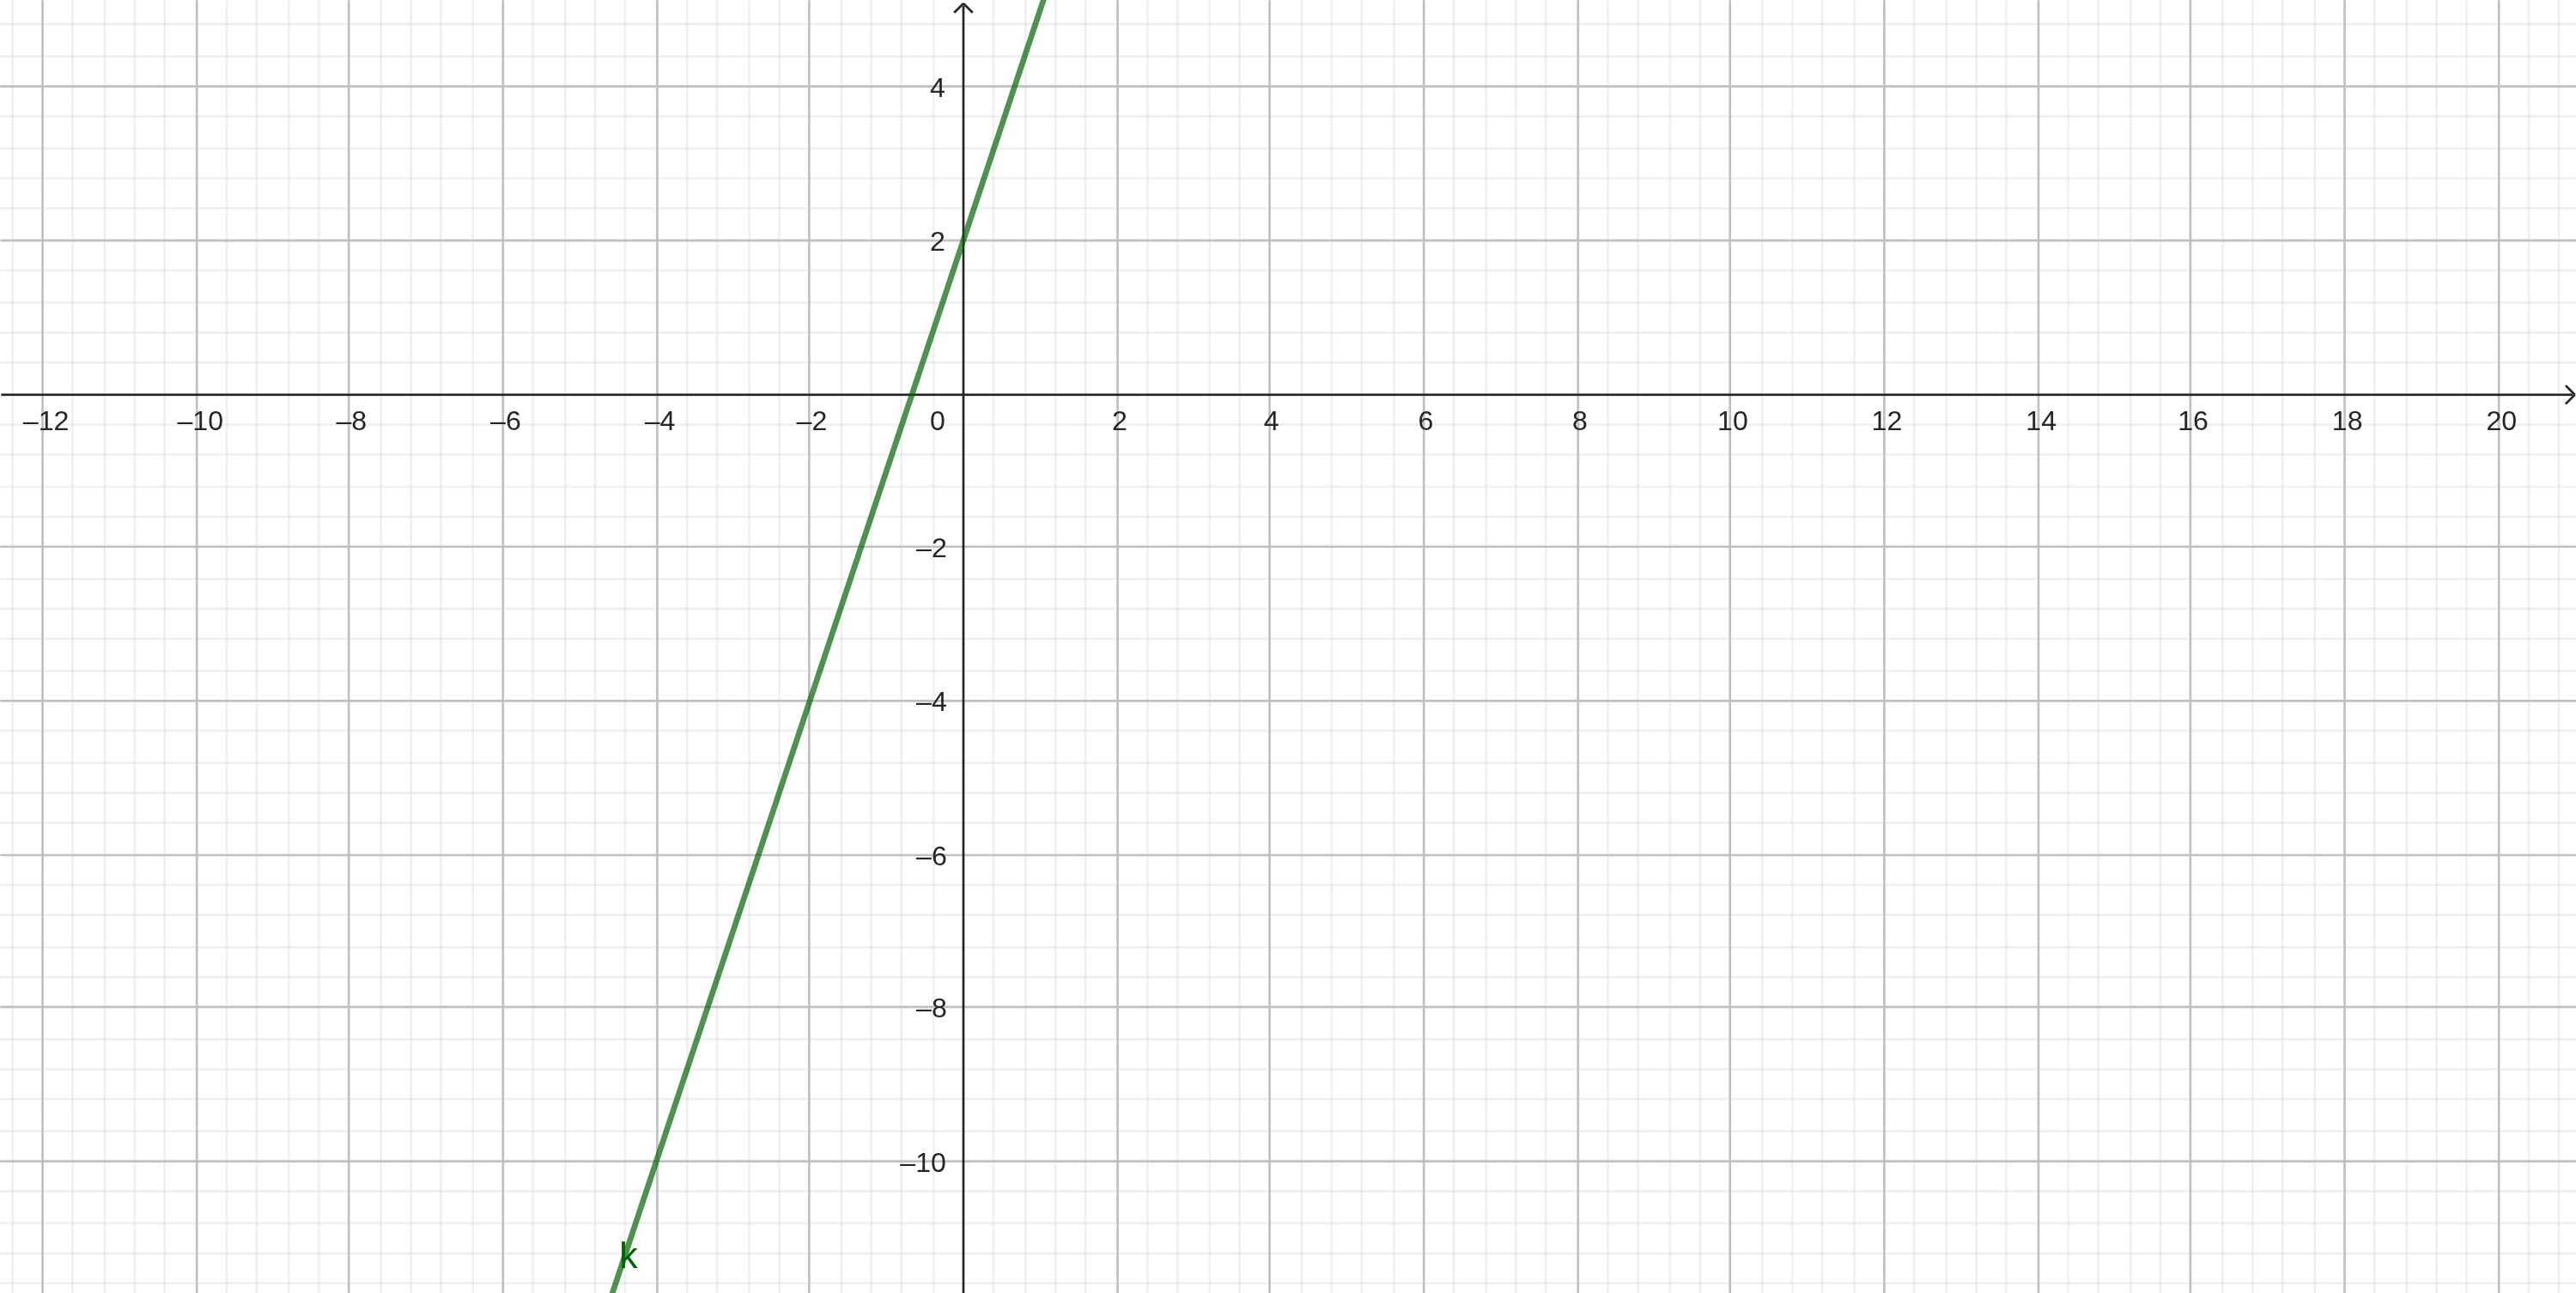
\includegraphics[width=0.8\textwidth]{Compo2ndLDroiteAffine}
\caption{Représentation graphique de la droite}
\label{fig:monimage}
\end{figure}
\href{https://www.geogebra.org/classic/erty3fcq}{Clique ici pour voir la courbe sur géogébra}\\
\end{center}

    \end{enumerate}
\end{enumerate}


\vspace{0.5cm}

\subsection*{\underline{PARTIE B :} 3 pts}

\begin{enumerate}
    \item Les droites \((D)\) et \((D')\) ont pour équations :
    \[
    (D) : y = -7x + 8 \quad \text{et} \quad (D') : y = -7x + 2
    \]

    Ce sont deux droites de la forme \( y = ax + b \), avec \( a = -7 \) dans les deux cas.

    \textbf{Conclusion :} Elles ont le même coefficient directeur \( \Rightarrow \) elles sont \textbf{parallèles}.

    \[
    \boxed{(D) \parallel (D')}
    \]

    \item On cherche la valeur de \( m \) pour que la droite \( (D_1) : y = mx + 2 \) soit parallèle à \( (D_2) : 4x - 2y + 3 = 0 \)

    Réécrivons \( (D_2) \) sous la forme \( y = ax + b \) :

    \[
    4x - 2y + 3 = 0 \quad \Leftrightarrow \quad -2y = -4x - 3 \quad \Leftrightarrow \quad y = 2x + \frac{3}{2}
    \]

    Donc la pente de \( (D_2) \) est \( a = 2 \)

    Pour que \( (D_1) \parallel (D_2) \), il faut \( m = 2 \)

    \begin{resultbox}
    \[
    \mathbf{m = 2}
    \]
		\end{resultbox}
\end{enumerate}



\end{document}